%%%%%%%%%%%%%%%%%%%%%%%%%%%%%%%%%%%%%%%%%
% Stylish Article
% LaTeX Template
% Version 2.1 (1/10/15)
%
% This template has been downloaded from:
% http://www.LaTeXTemplates.com
%
% Original author:
% Mathias Legrand (legrand.mathias@gmail.com) 
% With extensive modifications by:
% Vel (vel@latextemplates.com)
%
% License:
% CC BY-NC-SA 3.0 (http://creativecommons.org/licenses/by-nc-sa/3.0/)
%1
%%%%%%%%%%%%%%%%%%%%%%%%%%%%%%%%%%%%%%%%%

%--------------------------------------------------------------# Path to your oh-my-zsh installation.--------------------------
%	PACKAGES AND OTHER DOCUMENT CONFIGURATIONS
%----------------------------------------------------------------------------------------

\documentclass[fleqn,10pt]{SelfArx} % Document font size and equations flushed left

\usepackage[english]{babel} % Specify a different language here - english by default

\usepackage{marvosym, epigraph, subfig, listings, microtype}

\usepackage[sortcites=false,style=authoryear-comp,bibencoding=utf8, natbib=true, firstinits=true, maxcitenames=2, maxbibnames = 99, uniquename=false, backend=bibtex, useprefix=true, backref=false,doi=false,isbn=false,url=false,dashed=true]{biblatex}
\setlength\bibhang{20pt}
\bibliography{references.bib}
\AtEveryBibitem{%
	\clearfield{day}%
	\clearfield{month}%
	\clearfield{endday}%
	\clearfield{endmonth}%
}

%----------------------------------------------------------------------------------------
%	COLUMNS
%----------------------------------------------------------------------------------------

\setlength{\columnsep}{0.55cm} % Distance between the two columns of text
\setlength{\fboxrule}{0.75pt} % Width of the border around the abstract

%----------------------------------------------------------------------------------------
%	COLORS
%----------------------------------------------------------------------------------------

\definecolor{color1}{RGB}{0,0,90} % Color of the article title and sections
\definecolor{color2}{RGB}{0,20,20} % Color of the boxes behind the abstract and headings

%----------------------------------------------------------------------------------------
%	HYPERLINKS
%----------------------------------------------------------------------------------------

\usepackage{hyperref} % Required for hyperlinks
\hypersetup{hidelinks,colorlinks,breaklinks=true,urlcolor=color2,citecolor=color1,linkcolor=color1,bookmarksopen=false,pdftitle={Housing market and migration revisited: a Bayesian multilevel gravity model for Dutch municipalities},pdfauthor={Thomas de Graaff}}

%----------------------------------------------------------------------------------------
%	ARTICLE INFORMATION
%----------------------------------------------------------------------------------------

\JournalInfo{Conference paper} % Journal information 
\Archive{Prepared for ERSA 2019} % Additional notes (e.g. copyrigh, DOI, review/research article)

\PaperTitle{Housing market and migration revisited: a Bayesian multilevel gravity model for Dutch municipalities}

\Authors{Thomas de Graaff\textsuperscript{1}*} % Authors
\affiliation{\textsuperscript{1}\textit{Department of Spatial Economics, Vrije Universiteit Amsterdam, Amsterdam, The Netherlands}} % Author affiliation
\affiliation{*\textbf{Corresponding author}: \Letter{} t.de.graaff@vu.n; \Mundus{} \href{thomasdegraaff.nl}{thomasdegraaff.nl}} % Corresponding author

\Keywords{Gravity model --- housing market --- migration --- multilevel model --- partial pooling --- prediction}
\newcommand{\keywordname}{Keywords} 

%%----------------------------------------------------------------------------------------
%%	ABSTRACT
%%----------------------------------------------------------------------------------------

\Abstract{By applying a Bayesian multilevel gravity model, this paper
  revisits the impact of home-ownership and social renting rates on
  intercity migration. Where most of the extant literatures focuses on
  using fixed effects for cities of origin and destination, I adopt a
  Bayesian multilevel approach. This approach has two main
  advantages. First, it allows for simultaneous estimation of city
  specific effects and the effects of city specific home-ownership and
  social renting rates on migration flows, where the impact is not
  necessarily symmetrical for cities of origin and
  destination. Second, it allows for prediction of migration flows
  between cities both in- and out-of-sample. The results show that
  home-ownership rates decrease migration flows significantly with an
  elasticity below $-1$. Municipal social renting rate has a negative
  impact as well, but its elasticity is close to zero. I use these
  estimates to predict changes in all in- and out-going migration flows in
  Amsterdam driven by an increase in the home-ownership rate. }

%----------------------------------------------------------------------------------------
\hypersetup{draft} 
\begin{document}
	
	\flushbottom % Makes all text pages the same height
	\maketitle % Print the title and abstract box
	%\tableofcontents % Print the contents section
	\thispagestyle{empty} % Removes page numbering from the first page
	
	%----------------------------------------------------------------------------------------
	
	\section{Introduction} % The \section*{} command stops section numbering

        The current Dutch housing market is characterized by a low
        housing supply elasticity, high housing demand, and only a
        small segment (10\%) that belongs to the private rental market
        \citep{michielsen2017}. Because of the resulting large
        shortage of housing, many policy recommendations have been
        proposed, including plans for 700,000 new houses to be built
        in the coming decade. Unfortunately, the construction of a
        large amount of new dwellings is problematic in the
        Netherlands due to large and restrictive spatial constraints
        \citep{michielsen2019}. Therefore, policy makers consider 
        as well to change the housing structure, e.g., by converting
        rent controlled housing to home-ownership properties, to
        tackle at least the high housing prices by enlarging the
        home-ownership segment.
        
        There is already a large amount of literature looking into the positive
        and negative effects of home-ownership---both from a private and from a social perspective \citep[see for an
        overview][]{dietz2003social}. It is argued that home-ownership leads to,
        e.g., better maintenance (of the own dwelling and the neighbourhood),
        more savings, higher education outcomes, higher individual labor supply,
        and even better health. One prominent negative effect of home-ownership
        is that it leads to less incentives to move residence because of higher
        moving costs vis-\`{a}-vis private renting.  
        
        This paper revisits the role of housing market structure as impediment
        for inter-municipality migration and specifically focuses on the role of
        home-ownership and social renting rates. In addition, it gives a
        framework to predict changes in the whole network of migration flows,
        when housing market structure change locally.  To this end, I adopt a
        Bayesian multilevel gravity model which is not frequently encountered in
        the traditional gravity literature.\footnote{That is, in the economic
          literature; a notable exception is \citet{ranjan2007bayesian} in the
          economic trade literature. In the geographical literature this
          approach is more commonly adopted \citep[see within a migration
          context][]{congdon2010random, congdon2012spatial}} Traditional gravity
        modelling has the disadvantage that either municipality fixed effects of
        origins and destinations can be incorporated or the municipalities'
        characteristics when not varying over flows. This paper circumvents this
        disadvantage by adopting a multilevel approach with partial
        pooling\footnote{There is a whole variety of names for these types of
          models, including hierarchical modeling, varying effects, mixed
          effects and shrinkage models. I use the more generic multilevel
          description as municipality and flows are by definition measured at a
          different level (scale) \citep[see][for an indepth
          discussion]{gelman2013bayesian}.}, where the latter terms indicates
        that I do not impose fixed effects to control for origin and destination
        specific effects, but that I ``draw'' them from a distribution, hence
        the name partial pooling (where complete pooling states no group effects
        and no pooling fixed effects).
               
        This papers adds two main elements to the literature. First, it does not
        only consider home-ownership but as well municipal social renting
        structure, which can be argued \citep[see, e.g.,][]{hughes1981council,
          boyle1997public,boyle1998migration} to have a large effect on regional
        mobility as well as social renting rights are usually only valid locally
        (within municipality) and are lost when moving residence between
        municipalities.
        
        Second, a partial pooling approach has another advantage, namely the
        municipal varying effects are completely probabilistic, making it
        feasible to predict both within and out-of-sample. In other words, with
        the results at hand I can predict migration flows between existing
        \emph{and} hypothetical cities. The former might be used for looking at
        counterfactuals; for example, the changes in in-migration for all
        municipalities, when one municipality changes its housing structure. The
        latter is useful when one wants to assess new migrations flows between
        one or even two new municipalities outside the sample.\footnote{See for
          probabilistic predictions of internation migration
          \cite{azose2015bayesian}.}
	
    	That housing market structure has a sizeable effect on migration
    	decisions is empirically well-established, especially at the
    	micro-level, where it is widely accepted that home-ownership has a
    	negative effect on municipal mobility \citep{dietz2003social,
    		dohmen2005housing}. For example, \citet{palomares2018understanding}
    	find that home-ownership has a very strong immobility effect on internal
    	migration in Spain during the period 2001--2011.
    	
    	In the literature, less attention has been given to inter-city
    	migration on the aggregate level with respect to the housing market as a
    	specific barrier.\footnote{See \citet{cushing2004crossing} for a
    		historical overview of common themes within migration research.} For
    	the UK, \citet{congdon2010random} found within a multilevel gravity
    	model that social rented housing had little effect on the attractivity
    	of a region, although it had a small positive effect on preventing
    	people from moving residence. For the Canadian case,
    	\citet{amirault2016drags} looked at the impact of home-ownership on
    	migration flows within a gravity model using a Poisson pseudo maximum
    	likelihood estimator and found an elasticity around $-1$.
    	           
        One of the main reasons to look into housing market structure and migration is that   
        higher moving costs are detrimental to the aggregate labor market
        \citep{oswald1996conjecture, oswald1999housing}. There is a large
        empirical literature \citep[see, e.g., ][]{munch2006homeowners,
          munch2008home, de2013european} looking at the impact of individual and
        aggregate home-ownership on labour market performance, where seemingly
        paradoxically at the aggregate level home-ownership is indeed harmful
        for labour market behaviour where at the individual level it is
        correlated with positive labour market performance.
        
        This difference between individual and aggregate level is explained by
        sorting. Home-owners are indeed less mobile than private renters because
        of higher fixed and sunk moving costs which has a negative
        \emph{aggregate} effect on labour market performance. However,
        home-owners are different from renters as they do \emph{individually}
        better on the labour market (due to individual unobserved
        heterogeneity). So home-owners in countries with high home-ownership
        rates perform worse on the labour market vis-\`a-vis home-owners in
        countries with low home-ownership rates; but they still perform better
        than private renters. For social renters, the effect is different from
        private renters. On the individual level they are less mobile than
        renters at the free market as well, but their labor market performance
        is also worse than that of private renters \citep{hughes1981council,
          de2009homeownership}.
        
        To anticipate the results of this paper, I find strong negative effects
        of home-ownership rates on inter-municipal migration flows. Further,
        social renting rates also affect migration flows negatively, but the
        effect is far less pronounced than for home-ownership and overlaps zero
        to a large extent. A possible interpretation of this finding is that
        those who sort into social renting are by definition less mobile than
        those who sort into home-ownership \citep[this argument is put forward
        by][as well]{boyle1998migration}. Finally, my model predicts that a 0.1
        increase in the rate of home-ownership in Amsterdam leads to an decrease
        of 8770 migrants into the city, 5890 migrants out of the city, and
        significant changes as well in the neighbouring municipaties.

        This paper reads as follows. The next section describes the data and
        focuses especially on the distribution of municipal migration flows and
        housing market structure. Section 3 describes the modelling
        approach, where starting from traditional gravity model and using the
        descriptives of the migration flows, a Bayesian multilevel gravity model
        is constructed. Section 4 gives both the model results and interprets
        them by providing as well predictions within and out-of-sample. The last
        section concludes.
        
        \section{Data}

        \begin{figure*}[t!]\centering % Using \begin{figure*} makes the figure take up the entire width of the page
          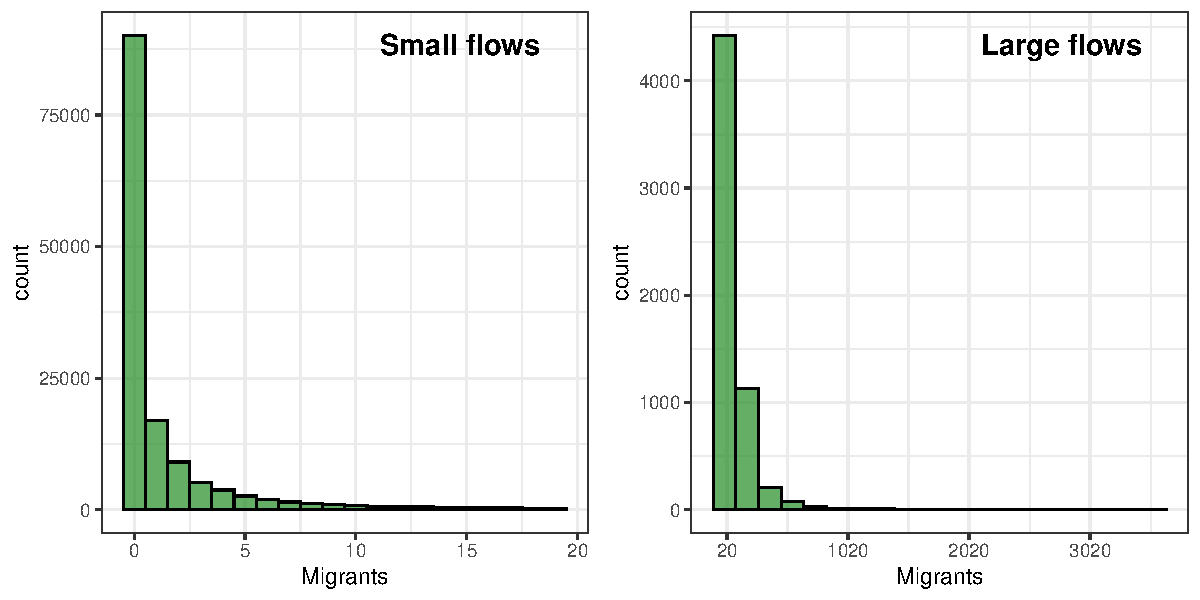
\includegraphics[width=0.8\linewidth]{../fig/hist_mig.pdf}
          \caption{Histogram of migrant flows. Left panel shows the
            histogram of small migrant flows ($0 \leq N < 20$) and the right
            panel shows the histogram of large migrant flows
            ($N \geq 20$). Note the different scale of the y-axes.}
          \label{fig:hist_mig}
        \end{figure*}

        I use inter-municipal migration flows measured in individuals
        between all of the 393 Dutch municipalities in 2015. There
        is no information available on within municipality residential
        migration. So, I have 393 municipal characteristics (or doubled
        when accounting for both origin and destination municipalities)
        and 154,056 aggregate migration flows ($393 \times 393 - 393$).

        The histograms in Figure \ref{fig:hist_mig} show the distribution of migrant
        flows within my sample. The left panel deals with migrant
        flows below 20, the right panel with migrant flows of 20 and
        larger. Two main observations can be made.

        First, there is strong but consistent decay in migration flow size in both panels,
        which points to a persistent underlying pattern. However, the
        right `tail' in this distribution is rather thick.\footnote{The
          largest migration flows are between the municipalities of
          Amsterdam and Amstelveen and amount to about 3,500
          migrants in 2015.} Thus, there are still observations quite far
        right in the distribution. Indeed, the sample mean is about
        10, while the sample variance is around 40, leading to a
        strong presence of \emph{overdispersion} (unconditional on
        other explanatory variables).  Second, two thirds of the
        dataset consists of zero observations. Although they do seem
        to be genuine observations and not caused by another process
        (I will check this by estimating a zero-inflated model as well),
         the occurrence of zeros does need to be taken
        specifically into account.

        Zeven explanatory variables are added to the model. First, to account for
        spatial distance decay between origin $i$ and destination $j$,
        distance between all municipalities are calculated as
        Eucledian distance between centroids
        ($\text{dist}_{ij}$). Secondly, as municipality mass we use
        population size for both city of origin and city of
        destination (so $\text{pop}_i$ and $\text{pop}_j$). Finally,
        for housing market structure we use variables indicating
        percentage of homeownership ($\text{home}_i$ and
        $\text{home}_j$) and percentage of social renting
        ($\text{soc}_i$ and $\text{soc}_j$), again in both cities of
        origin and destination. Social renting in the Netherlands
        includes all kinds of rent controlled housing but typically
        involves local housing corporations offering housing to lower
        income households, where eligibility is based on (local)
        waiting lists. Both social renting and homeownership are
        assumed to impede regional mobility in the Netherlands as argued in
        \citet{de2009homeownership}.

        \begin{figure*}[ht]\centering % Using \begin{figure*} makes the figure take up the entire width of the page
          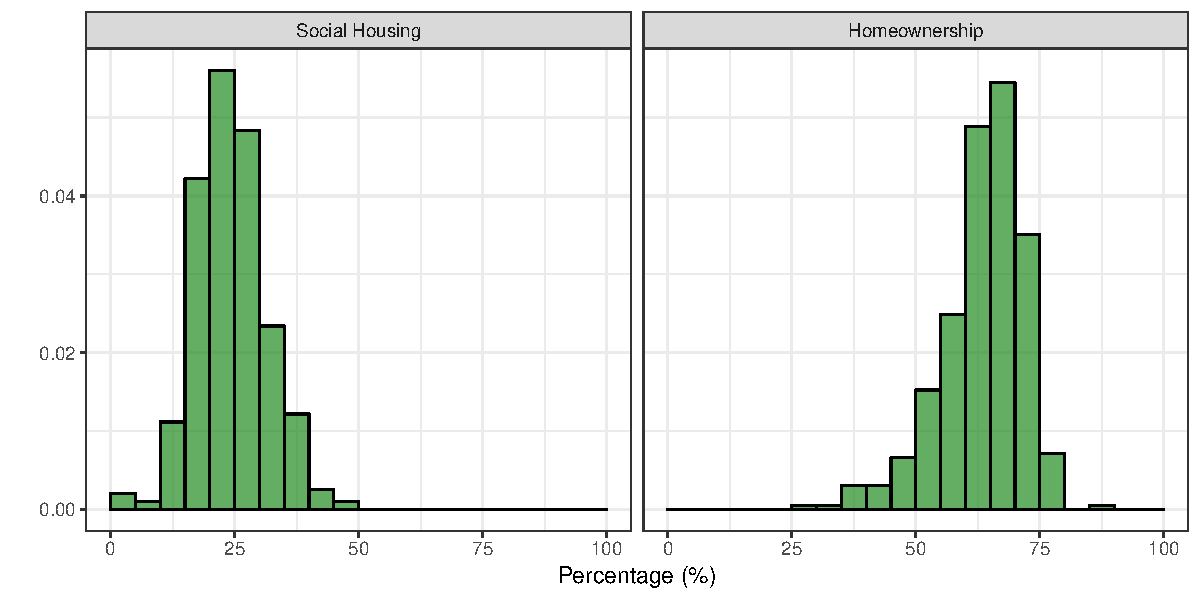
\includegraphics[width=0.8\linewidth]{../fig/hist_housing.pdf}
          \caption{Histogram of social housing (left) and
            homeownership (right) percentages in Dutch municipalities
            2015}
            \label{fig:housing_mig}
        \end{figure*}

        Figure \ref{fig:housing_mig} shows the distribution of social renting
        and homeownership across Dutch municipalities in 2015.  Clearly, both
        home-ownership and social housing are prevalent across Dutch
        municipalities, with an average per city of 25\% of social housing and around
        60\% of homeownership
    	Moreover, it is worthwhile to note that social
        renting is especially prevalent in the larger cities with a correlation
        of 0.4 between city size and social renting (e.g., Amsterdam has about a
        40\% social renting rate). Also, some smaller dutch municipalities do
        not exhibit any social renting. Homeownership and city size correlate
        negatively ($-0.51$). Finally, there is a large negative correlation
        between social renting and homeownership ($-0.84$) across
        municipalities.
        
        \section{Modeling framework}

        \subsection{The traditional gravity model}

        Throughout time, the workhorse model to study aggregate migration flows has been the gravity model (see \citet{anderson2011gravity} for a generic survey of the use of gravity models and \citet{poot2016gravity} for an overview of migration applications). I therefore start by adopting the basic gravity model specification pioneered by
        \citet{tinbergen1962shaping}, so:
        \begin{equation}
          \text{migrants}_{ij} = \text{M}_i^{\beta_1}\text{M}_j^{\beta_2}\text{dist}_{ij}^\gamma,
          \label{eq:grav}
        \end{equation}
        where $\text{migrants}_{ij}$ are the number of migrants going from $i$ to $j$, 
        $\text{M}_i$ ($\text{M}_j$) denotes the `mass' of $i$ ($j$), and $\text{dist}_{ij}$
        the distance between $i$ and $j$. Usually, the `mass' variables are proxied by population, gross domestic product, density, etcetera. Moreover, the variable
        $\text{dist}_{ij}$ may represent in general all sorts of frictions, not
        only physical distance.
        
        Importantly, \citet{anderson2003gravity} argued that origin
        and destination specific variables should be incorporated to
        take into account multilateral resistance terms. Most often,
        this is done by log-linearising model
        (\ref{eq:grav})\footnote{In our case, note that zeros are
          present in our social renting variable. We therefore add a
          small number to this variables (0.0001). Doing this only on
          the \emph{right-hand side} does only marginally affect our results.} and
        incorporating fixed effects for origins and destinations, as
        follows:
        \begin{equation}
          \log(\text{migrants}_{ij}) = o_i + d_j +  \gamma\log(\text{dist}_{ij})
          \label{eq:gravfixed}
        \end{equation} 
        Note that now all origin and destination specific variables are absorbed
        by the fixed effects $o_i$ and $d_j$ and that only variables affecting
        the frictions $(\text{dist}_{ij})$ can be incorporated.\footnote{If
          there is another variable dimension---say, repeated observations over
          time---then this might be circumvented. However, this requires enough
          variation in the data as time-invariant variables can still not be
          taken into account.}\footnote{An often applied strategy is to use
          differences between origin and destination specific variables. Take
          for example $\Delta h_{ij}$ as the difference in home-ownership rates
          between $i$ and $j$. A disadvantage of this approach is that the
          difference between 10\% and 20\% home-ownership rates and the
          difference between 80\% and 90\% home-ownership rates would be valued
          as the same.}
        \begin{figure}[ht]\centering 
        	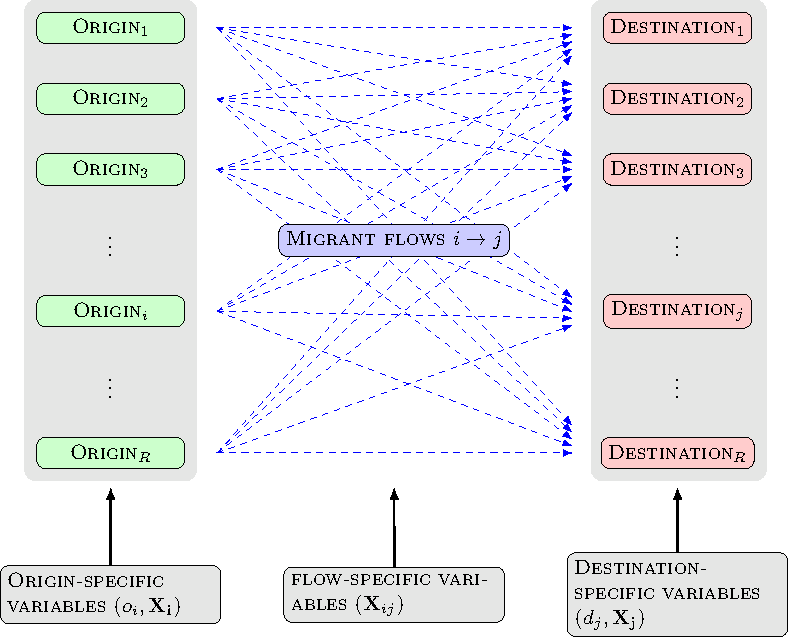
\includegraphics[width=\linewidth]{../fig/gravity_network.pdf}
        	\caption{Decomposition of variables impacting migration flows from $i$ to $j$ $\left(\{i,j\} \in \{1,\ldots, R\}\right)$}
        	\label{fig:gravity_network}
        \end{figure} 
        Figure \ref{fig:gravity_network} denotes the problem schematically in a
        generic dyadic type of network. Typically, one wants to model migration
        flows between $i$ and $j$, whilst taken into account both the municipal
        specific effects ($o_i$ and $d_j$) and the municipal variables
        ($\mathbf{X}_i$ and $\mathbf{X}_j$) one is interested in, such as
        housing market, population structure or cultural variables.
                  
        Moreover, equation (\ref{eq:gravfixed}) is typically estimated with
        linear regression type of models, which is often very cumbersome given
        the large amount of zeros migrants flows. `Quick and dirty' remedies as
        adding a small amount to the flow variable or removing all zeros have
        been proven to seriously bias the results \citep{linders2006estimation,
          burger2009specification}.
        	

        Therefore, I next allow for a different strategy, where I would like to
        tackle simultaneously the two disadvantes of above: incorporating both
        city varying effects and city specific variables and modelling the
        distribution of migrants flows as they are displayed in Figure
        \ref{fig:hist_mig}---even when being zero.

        \subsection{A Bayesian multilevel gravity model}

        First, as municipal migrants flows are discrete, non-negative and
        relatively rare give the size of the population, theoretically the most
        appropriate way to go forward is to model migrant flows with a Poisson
        type of model. However, given that the sampling variance is four times
        the sampling mean of the migration flows (although not conditional on
        the covariates), we likely need to correct for overdispersion of
        heteroskedasticity \citep[][states that heteroskedasticity (rather than
        the presence of too many zeros) is responsible for the main source of
        bias within gravity models.]{silva2006log}. An often used distribution
        to account for overdispersion is the Gamma-Poisson model (which is under
        re-parametrization similar to the perhaps better known negative binomial
        model). So, we use that for our outcome variable.

        To account for the multiplicative nature of the theoretical model as in
        (\ref{eq:grav}), I adopt a log link for the expected number of migrants
        $\lambda_{ij}$ in the Gamma-Poisson model.  Apart from the theoretical
        model, note that this log link ensures as well that the expected number
        of migrants is always positive.  Further, I assume that
        $\log(\lambda_{ij})$ is a linear function of the municipal specific
        variables and the distance between $i$ and $j$.

        Finally, to adopt both municipality effects and variables I adopt a
        multilevel model with partial pooling. This entails that the municipal
        varying effects (unlike fixed effects) are now drawn from a, in this
        case Normal, distribution, where the parameters of this distribution are
        estimated as well (in the Bayesian literature they are known as well as
        hyper-parameters).  Intuitively, this entails that municipalities are
        partially pooled indicating that (statistical) information between
        municipalities is shared. This is an attractive feature, as fixed
        effects assume no pooling. In that case, the model only learns from the
        information contained in that specific municipality whereas with partial
        pooling it is ensured that outliers (very high or low effects) are
        effectively \emph{shrunk} towards the mean. Indeed, this is a further
        extension of that best feature of linear regression: regression towards
        the mean.

        The complete model now looks as follows:\footnote{I adopt here the model structure from \citet{mcelreath2018statistical}.}
        
        \begin{subequations}
          \begin{align} \text{Migrants}_{ij} \sim & \text{Gamma-Poisson}(\lambda_{ij}, \tau) \label{outcome}\\
            \log(\lambda_{ij}) =
            & \alpha + o_{\text{mun}[i]} + d_{\text{mun}[j]} + \notag
            \\ & \beta_1 \log(\text{pop}_i) +
            \beta_2\log(\text{pop}_j) + \notag \\ & \beta_3
            \log(\text{home}_i) + \beta_4 \log(\text{home}_j) + \notag\\
            & \beta_5 \log(\text{soc}_i) + \beta_6 \log(\text{soc}_j)
            + \notag \\ & \beta_7 \log(\text{dist}_{ij}) \label{linear} \\
            o_{\text{mun}} \sim& \text{ Normal}(0, \sigma_o) \label{muno} \\
            d_{\text{mun}} \sim& \text{ Normal}(0, \sigma_d) \label{mund} \\
            \beta_1,\ldots, \beta_7 \sim& \text{
                                          Normal}(0,2)\\ \alpha_o, \alpha_d \sim& \text{ Normal}(0,2)\\
            \sigma_o, \sigma_d \sim& \text{ HalfCauchy}(0,1) \\ \tau
            \sim& \text{ Gamma}(0.01, 0.01)
          \end{align}
          \label{model}
        \end{subequations}
        The first part ({\ref{outcome}) models the outcome variable, being the
          number of migrants, using a Gamma-Poisson distribution (with parameter
          $\lambda_{ij}$) allowing for overdispersion by using an additional
          parameter $\tau$. The linear part of the model is given by
          (\ref{linear}) and states that the poisson outcome variable is on a
          log-scale and that most explanatory variables are on a log-scale as
          well, allowing for direct comparison of the parameters being
          elasticities. Equations (\ref{muno}) and {(\ref{mund}) constitute the
            multilevel part, where parameters $\sigma_o$ and $\sigma_d$ measure
            the amount of pooling. If they go to zero, then the data exhibits
            complete pooling. If they become very large (go to infinity) there
            is no pooling (which is the fixed effects case). Equations
            (3e)--(3h) denote priors for all parameter involved.  These priors
            are chosen that they are rather conservative. Namely, we know from
            previous empirical literature that the $\beta$-parameters typically
            are not lower than $-2$ or higher than $2$. But given the amount of
            data these priors are of little influence. The only structure I
            impose is that the standard deviations $\sigma_o$ and $\sigma_d$ are
            assumed to be non-negative with relatively probability in the their
            right tails. The Gamma prior for $\tau$ is a standard and as well a
            very conservative prior.
                      
        \section{Results}

        \subsection{Parameter estimates}
        
        Model (\ref{model}) is estimated by using the \emph{No U-Turn Sampler}
        (NUTS) from the Stan platform for statistical modeling and
        high-performance statistical computation.\footnote{See
          \href{https://mc-stan.org/}{https://mc-stan.org/}. As interface to
          Stan \citep[see for an overview article of Stan][]{carpenter2017stan}
          I used the R-package \texttt{brms} \citep{brms}.} NUTS is a relatively
        recent developed Hamiltonian Monte Carlo (a specific form of Markov
        Chain Monte Carlo simulation) method, able to draw samples efficiently
        from large multilevel models \citep{hoffman2014no}. Parameter estimates
        and probability intervals of the main parameters (so not the
        municipality specific effects: there are 786 of them) are given in Table
        \ref{tab:coef}. Perhaps more insightful, they are as well graphically
        depicted in Figure \ref{fig:forestplot}.

% latex table generated in R 3.4.4 by xtable 1.8-3 package
% Fri Feb 22 15:07:02 2019
\begin{table}[ht]
  \centering
  \caption{Parameter estimates with 95\% probability intervals (group specific origin and destination estimates are not presented)}
  \label{tab:coef}
  \begin{tabular}{lrrrr}
    \toprule
    Parameter & mean & sd & 2.5\% & 97.5\% \\ 
    \midrule
    Intercept      & $-0.74$ & 0.04 & $-0.82$ & $-0.66$ \\ 
    log(pop$_i$)   & 0.89 & 0.03 & 0.83 & 0.96 \\ 
    log(pop$_j$)   & 0.88 & 0.04 & 0.79 & 0.97 \\ 
    log(home$_i$)  & $-1.48$ & 0.19 & $-1.86$ & $-1.10$ \\ 
    log(home$_j$)  & $-1.27$ & 0.25 & $-1.75$ & $-0.78$ \\ 
    log(soc$_i$)   & $-0.04$ & 0.04 & $-0.11$ & 0.03 \\
    log(soc$_j$)   & $-0.06$ & 0.03 & $-0.12$ & $-0.01$ \\ 
    log(dist$_{ij})$ & $-1.96$ & 0.01 & $-1.97$ & $-1.95$ \\ 
    $\sigma_o$    & 0.45 & 0.02 & 0.42 & 0.49 \\ 
    $\sigma_j$    & 0.61 & 0.02 & 0.57 & 0.66 \\ 
    $\tau$        & 1.22 & 0.01 & 1.20 & 1.24 \\ 
    \bottomrule
  \end{tabular}
\end{table}
\noindent Note again that both the outcome and the $\beta$-variables are on the
log scale, so they constitute elasticities.  Thus, population (both in city of
origin and of destination) has an elasticity of about 0.9 with migration. If
population doubles, migration increases by 90\%.  As expected, housing structure
indeed impedes municipal mobility, but it is primarily home-ownership rates and
not social renting rates that have a sizeable effect. Percentage home-ownership
in the city of origin has an elasticity of about $-1.5$ and in the city of
destination of $-1.3$ with migration. Social renting has a much smaller impact
with only an elasticity of about $-0.04$ in the city of origin and $-0.06$ in
the city of destination, but note the probability intervals overlap 0 to a
considerable extent. The home-ownership elasticities I find are slightly larger
in absolute size than what \citet{amirault2016drags} reported. The
distance-decay parameter is conform previous literature and is $-1.96$ The
latter is significantly larger in absolute value that typical parameters
reported by regression type of models, but is more in less line with parameters
estimated by negative binomial or poisson type of models.

Furthermore, if anything, the low values for the parameters $\sigma_o$ and
$\sigma_d$ point to more pooling than less, so fixed effects in this case could
lead to substantial overfitting.

\begin{figure}
  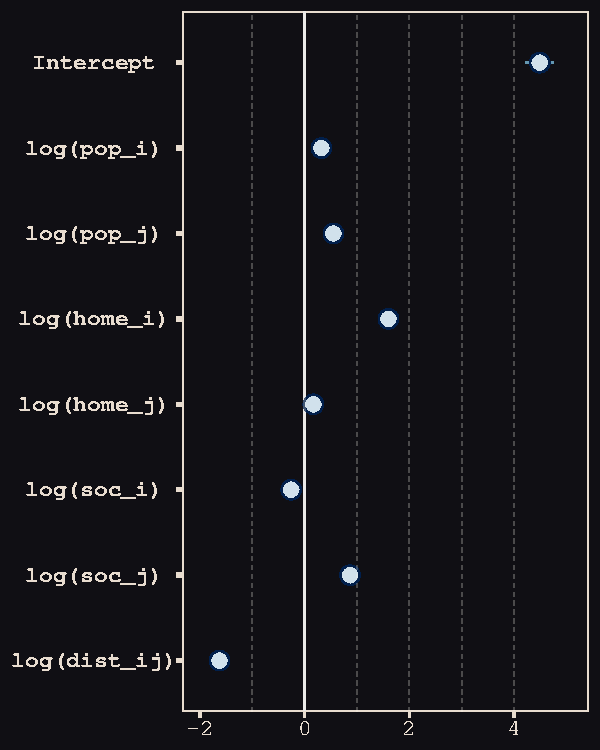
\includegraphics[width = \columnwidth]{../fig/forestplot.pdf}
  \caption{Forest plot of parameter means and 95\% probability
    intervals (group specific origin and destination estimates are not
    presented)}
  \label{fig:forestplot}
\end{figure}

For each municipality the models estimates as well an origin specific effect
($o_i$) and a destination specific effect ($d_j$). These are depicted in maps
\ref{fig:out} and \ref{fig:in} and can be interpreted as having relatively less
or more migration \emph{relative} to population size and housing structure.

\begin{figure}
		\centering
		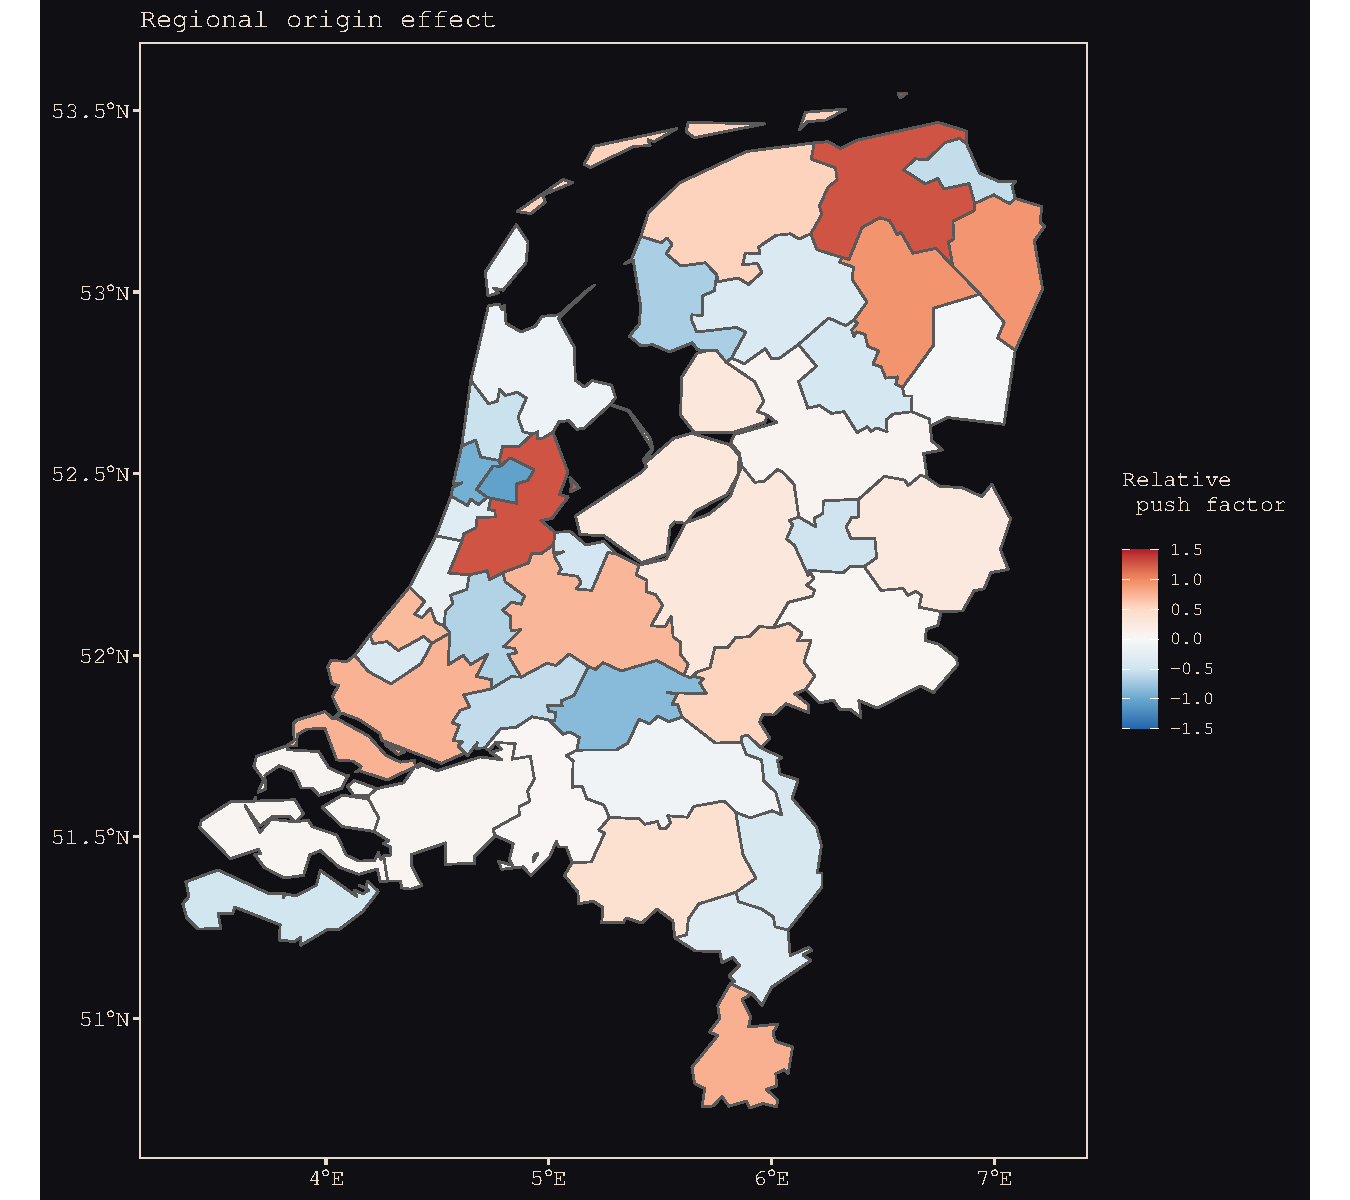
\includegraphics[width = \columnwidth]{../fig/p_coef_out.pdf}
		\caption{Municipality specific origin effects}\label{fig:out}
\end{figure}

Figure \ref{fig:out} first shows the municipal specific origin effects. Clearly,
there is a relatively larger push factor in the peripheral Dutch
municipalities. These are actually regions that loose population. The areas that
loose relatively few people are to be found in the Dutch core region (the
``Randstad'') including the largest Dutch cities: Amsterdam, Rotterdam, The
Hague and Utrecht.

\begin{figure}
	\centering
	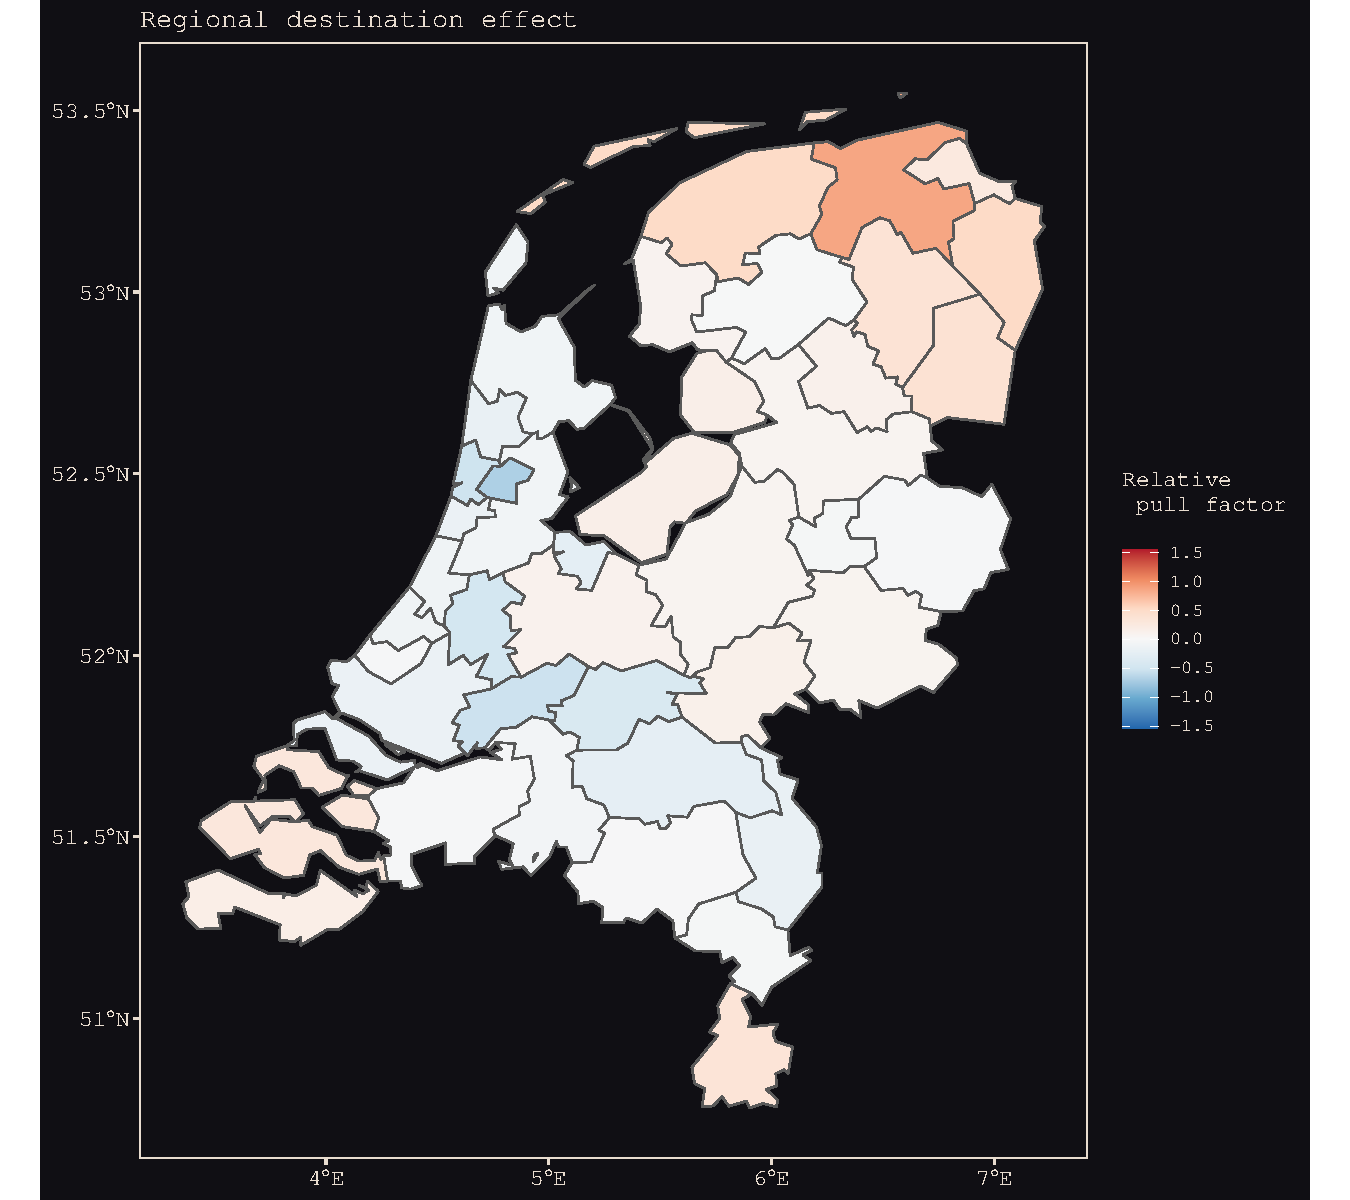
\includegraphics[width = \columnwidth]{../fig/p_coef_in.pdf}
	\caption{Municipality specific destination effects}\label{fig:in}
\end{figure}

Figure \ref{fig:in} shows the municipality specific destination
effects. Interestingly, these seem to mirror to a certain extent the
municipality specific origin effects. Again, relatively most people seem to move
to the peripheral municipalities---albeit to a lesser extent than the push
factor. That means that controlling for housing and population, relatively few
people move to the largest cities in the Netherlands. This is due to the
scarcity of available housing in that period (partly due to the housing
structure) and the fact that this model does not reflect price differences. The
``Randstad area'' in the Netherlands is very popular, but because of housing
shortage this is mainly reflected in higher prices and an increasingly tighter
housing market. Housing is still available in the least attractive regions of
the Netherlands and this is where most dynamics in terms of moving residence
take place. This indicates as well that the municipality specific destination
effects should not be interpreted as attractivity effects as, e.g., in
\citet{congdon2010random}.

Figures \ref{fig:out} and \ref{fig:in} indicates as well that the municipality
specific origin and destination effects are most likely highly
correlated. Moreover, given the facts that nearby municipalities often show
similar values, ideally both types of effects should be modelled as being
spatially autocorrelated.

\subsection{Model predictions}

\begin{figure*}[t!]\centering 
  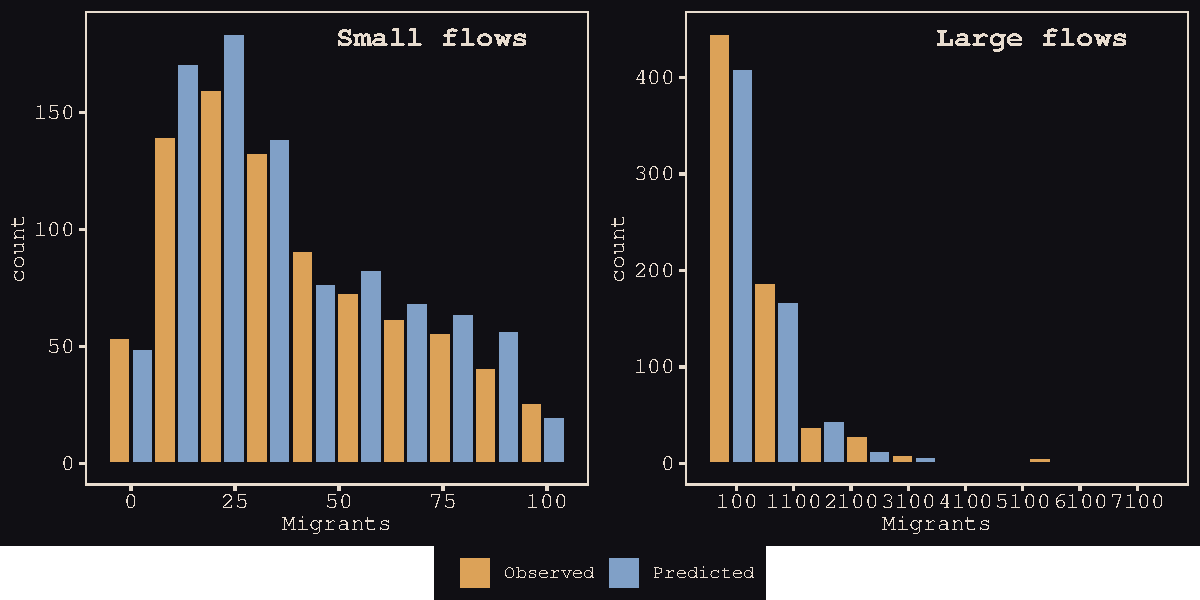
\includegraphics[width=0.8\linewidth]{../fig/hist_fit.pdf}
  \caption{Histogram of observed and predicted migrant flows. Left
    panel shows the histogram of small migrant flows ($0 \leq N < 20$)
    and the right panel shows the histogram of large migrant flows
    ($N \geq 20$). Note the different scale of the y-axes. Predicted
    migrant flows above 4,020 were removed for reasons of clarity and
    comparability with the observed migrant flows.}
  \label{fig:hist_fit}
\end{figure*}

To assess to what extent the model predictions are in line with the observed
data, Figure \ref{fig:hist_fit} shows the histogram of both observed and
predicted flows side by side. Eyeballing the evidence, it seems that the
distribution of predicted flows comes very close to the distribution of the
observed migration flows. The distribution of predicted migration flows seems
somewhat flatter though, as it predicts around 12,500 less zeros and more or
less the same amount more ones. What is not shown in the histogram (and if, it
would be very difficult to discern) is that the model predicts a couple of large
outliers---flows as large as 100,000 migrants. These outliers are mainly caused
by the city of Rotterdam, which has a large population and with 25\% only a very
small percentage of home-ownership. Even though these flows constitute a very
small percentage of total flows ($<$ 0.1\%), they are important in terms of
size. The underlying reason for this over-prediction is the homogeneous impact
of housing tenure on migration flows for all municipalities, regardless of
population size. It is quite likely that housing tenure in larger cities has a
different effect on migration than in smaller cities.

\begin{figure}
	\centering 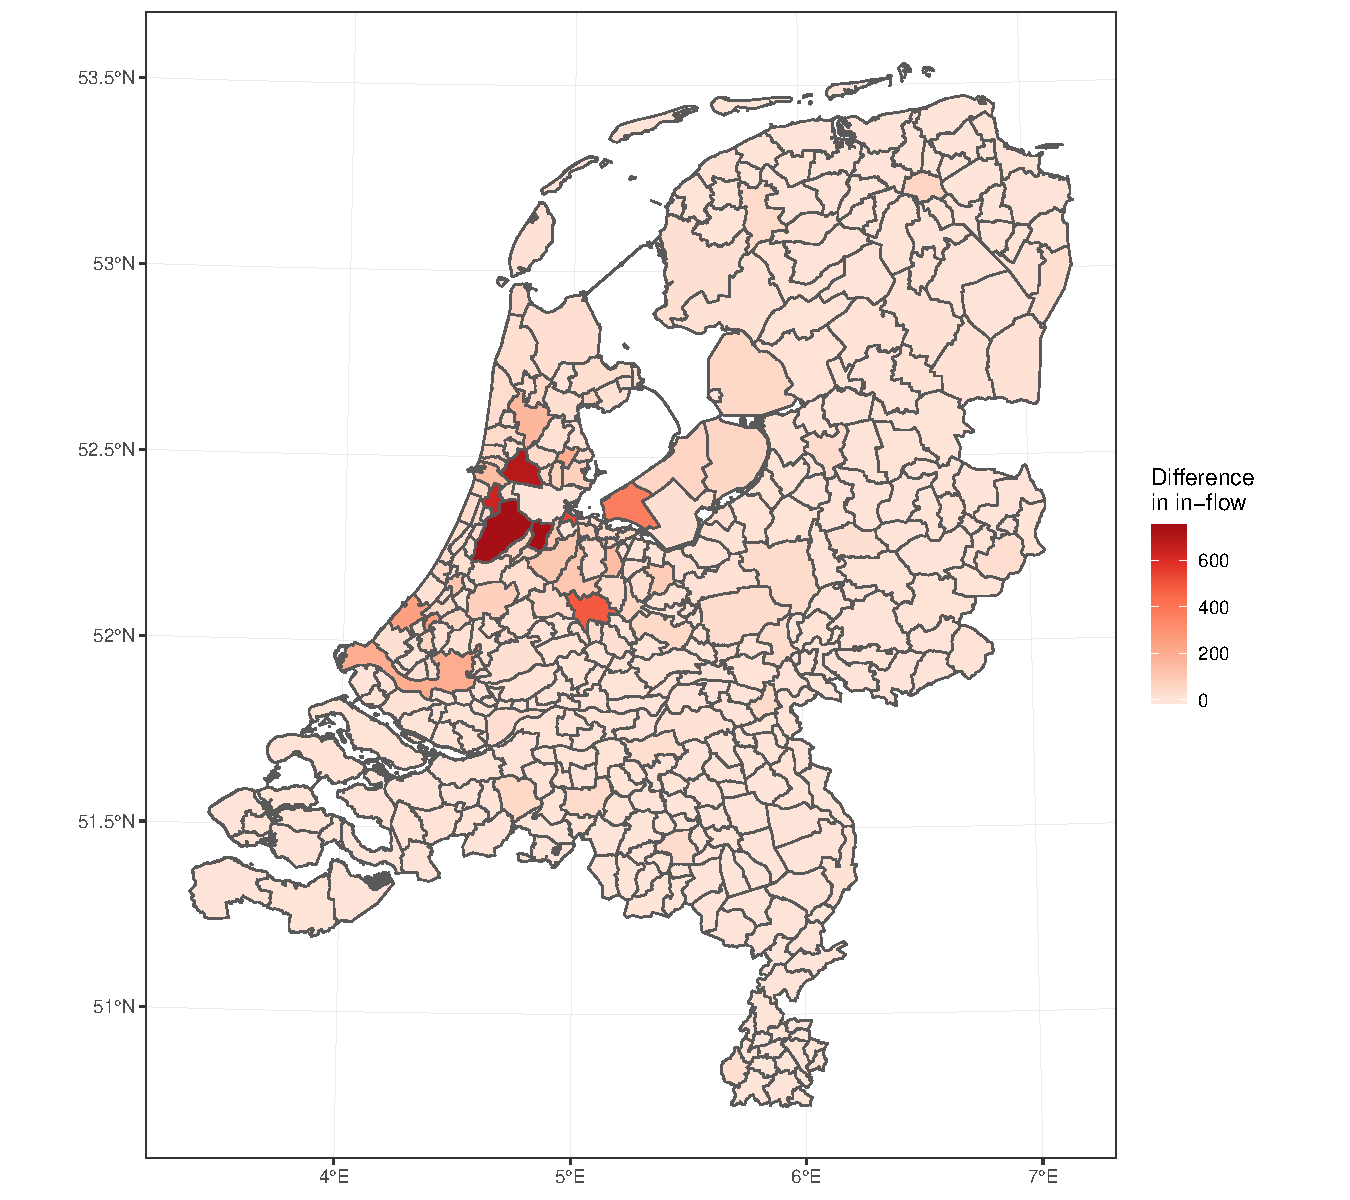
\includegraphics[width =
	\columnwidth]{../fig/p_diff_in.pdf}
	\caption{Changes in migrant flows into Amsterdam when percentage home-ownership
		in Amsterdam increases by 10 percentage points}\label{fig:diff_in}
\end{figure}

To assess what happens we look at the counterfactual when Amsterdam increases
its home-ownership rate with 10 percentage points---a large but not very
unrealistic scenario.  As a result, due to the large negative elasticities of
home-ownership, migration flows decrease significantly. Figure \ref{fig:diff_in}
shows the resulting difference in migration flows to Amsterdam.  The decrease in
flows range between 0 and 650, with the largest decreases from neighbouring
municipalities and from the larger cities in the Netherlands (Rotterdam, The
Hague and Utrecht). In total, in-migration drops with 8770 migrants.

\begin{figure}
  \centering 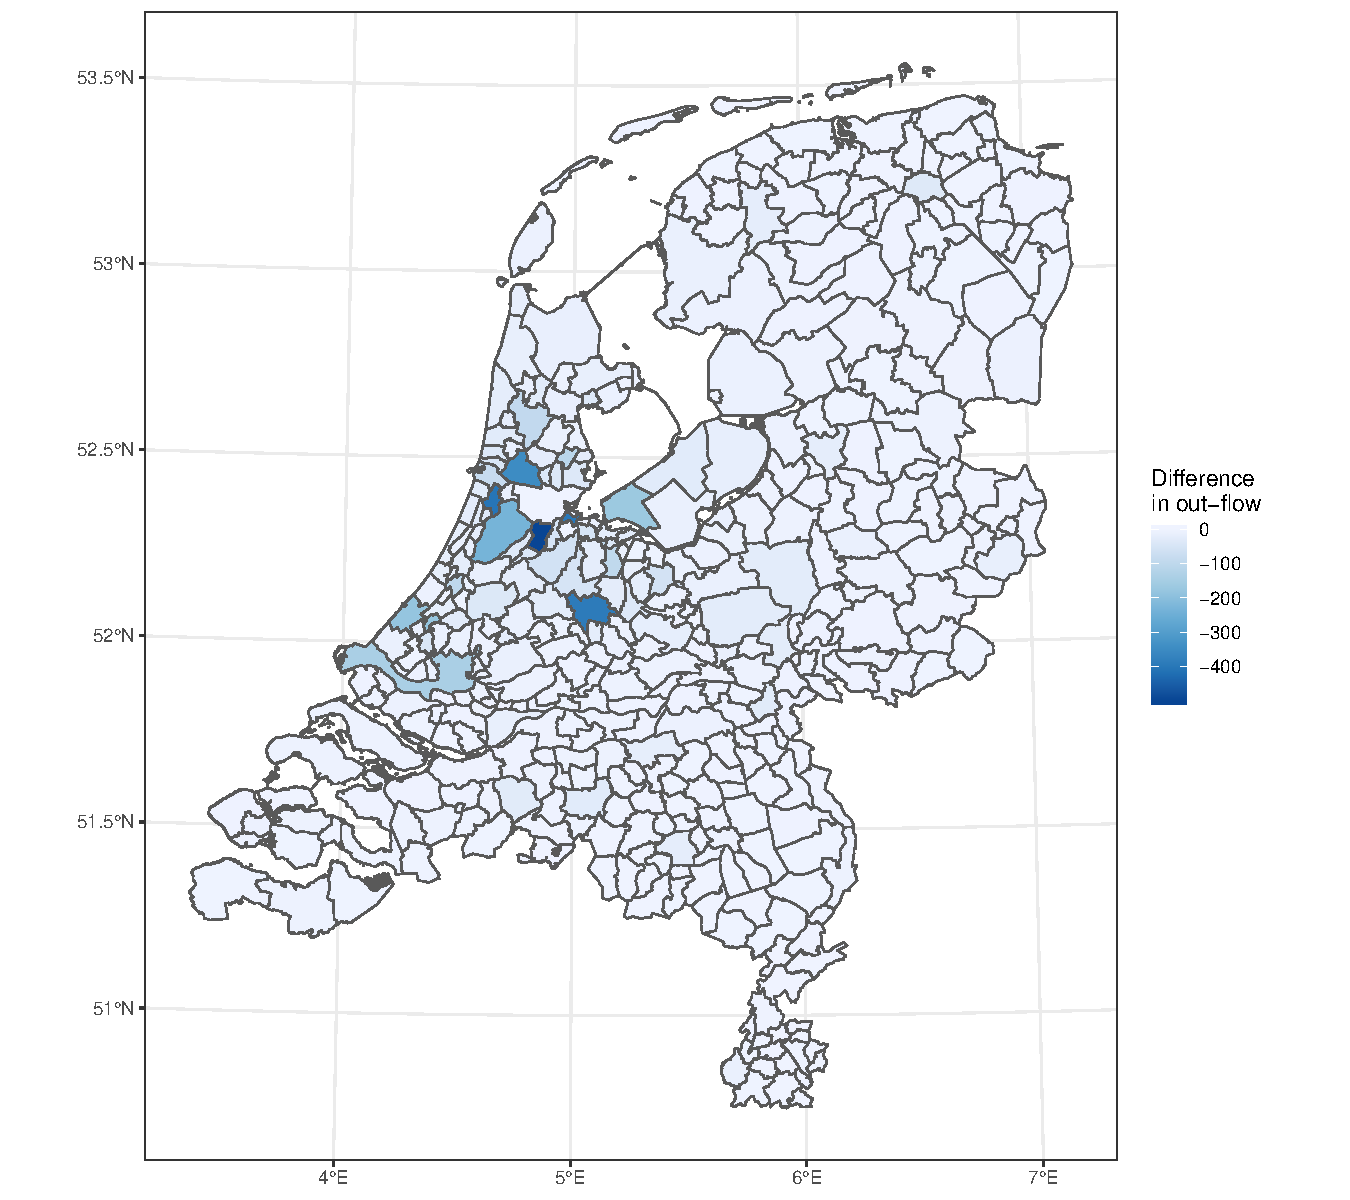
\includegraphics[width =
  \columnwidth]{../fig/p_diff_out.pdf}
  \caption{Changes in migrant flows from Amsterdam when percentage home-ownership
    in Amsterdam increases by 10  percentage points}\label{fig:diff_out}
\end{figure}

Figure \ref{fig:diff_out} shows the decrease in out-migration flows. The
decrease is slightly less and ranges between 0 and 500, with more or less
similar patters as Figure \ref{fig:diff_in}. Total out-migration drops now with
5892 migrants.

\section{In conclusion}

My goals with this paper are twofold. First, I revisit the impact of
home-ownership and social renting rates on intercity migration. Second, I seek
to provide a framework to produce predictions of intercity migration flows.  I
applied a Bayesian multilevel gravity model to accomplish these goals. The
resulting estimations are mostly in line with previous literature.  The distance
decay parameter is close to $-2$ and the parameters associated with the
population of origin and destination are both around 0.9.  Home-ownership turns
out to be a very important pull and push factors, having elasticities of $-1.48$
and $-1.27$, respectively. However, the impact of social renting is almost 0,
both for origin and destination. Thus, within this modelling framework social
renting structure neither works as pull or push factor, which is remarkable
given the fact that social renting right can only be acquired within the
municipality. \citet{boyle1998migration} draws a similar conclusion and argues
that social renters form a segment of the population that is not inclined to
move residence regardless the housing tenure. However, we observe that there is
a large correlation between city size and housing tenure---larger cities have
more social renting and less home-ownership. So, the average effect may be close
to zero but there could be huge variation over city size.

I show as well that the distribution of predicted migration flows is much in
line with that of the observed migration flows and that the model is capable of
predicting counterfactual flows when municipal housing structure changes. For
example, if the percentage of home-ownership in Amsterdam increase by 10
percentage points, migration flows in and out of amsterdam decrease with an
amount up to 600 migrants. Moreover, total inflow decreases with 8770 and total
outflows decreases with 5892 migrants.

Obviously, model refinements can be made. First, the model predicts a handful of
very large and unrealistic migrant flows (100,000 migrants) which are caused by
the city of Rotterdam which both has a large population and a very low amount of
home-ownership (25\%). At the moment the model still assumes a homogeneous
impact of housing tenure, which is unlikely given the strong correlation between
city size and housing tenure. To account for the likely heterogeneity of the
impact of housing tenure one can either incorporate interaction terms between
municipal population and housing tenure or impose varying effects in the
parameters of housing tenure. The latter approach is more likely to capture
heterogeneity but increases the amount of effective parameters considerably and
increases the complexity in interpreting the results.

Second, it is very plausible that the origin and destination effects,
$o_{\text{mun}[i]}$ and $d_{\text{mun}[j]}$, are highly correlated. Indeed, due
to institutions, sector structure, religion, etcetera, some municipalities may
be very open, whilst others may be very closed to outsiders. Allowing that these
effects are correlated could greatly increase model performance.

Third, and finally, nearby municipalities may be correlated in behaviour as
local labour market regions are typically larger than municipalities in the
Netherlands. Incorporating a spatial structure, e.g., in the varying regional
effects may further increase model performance by smoothing outliers
\citep[see][for an example]{congdon2010random}.

As Bayesian multilevel modelling is very flexible these further refinements of
the model can all be readily incorporated. The only restriction is computer
power as these types of models are not very scalable in observations or
parameters. At the moment, drawing a reasonable amount of samples requires
around six hours. On the other hand, a better model structure greatly improves
the efficiency of sampling, The only problem that most likely remains is
interpreting all results in an insightful and useful manner.

\section*{Acknowledgments} % The \section*{} command stops section numbering

I would like to thank Wim Bernasco and participants at the 15$^{th}$ biennial
NECTAR conference in Helsinki for valuable comments on a first draft of this
paper. Paper, data and code can be retrieved from the project's GitHub page:

\href{https://github.com/Thdegraaff/migration_gravity}{https://github.com/Thdegraaff/migration\_gravity}.
	%----------------------------------------------------------------------------------------
	%	REFERENCE LIST
	%----------------------------------------------------------------------------------------
	
	\addcontentsline{toc}{section}{references} % Adds this section to the table of contents
	\printbibliography
	
	%----------------------------------------------------------------------------------------
	
\end{document}
%%% Local Variables:
%%% mode: latex
%%% TeX-master: t
%%% End:
